%%%%%%%
% Ch5 %
%%%%%%%

\chapter{One-quadrant choppers - Switched-mode power supply (SMPS)}	
    For a single-quadrant DC/DC conversion, we can use simpler systems. The main application field is that of electronic equipments. Those equipments often need \textbf{galvanic isolation} in order to be employed safely. When the switch of the DC/DC converter works in on (closed state, almost short-circuit) off (open state, almost open-circuit), we call it \textbf{switched-mode power supply} (SMPS), as opposed to \textbf{linear supplies}.
	
	\section{Linear supplies versus SMPSs}
		\begin{wrapfigure}[12]{l}{5.5cm}
		\vspace{-5mm}
		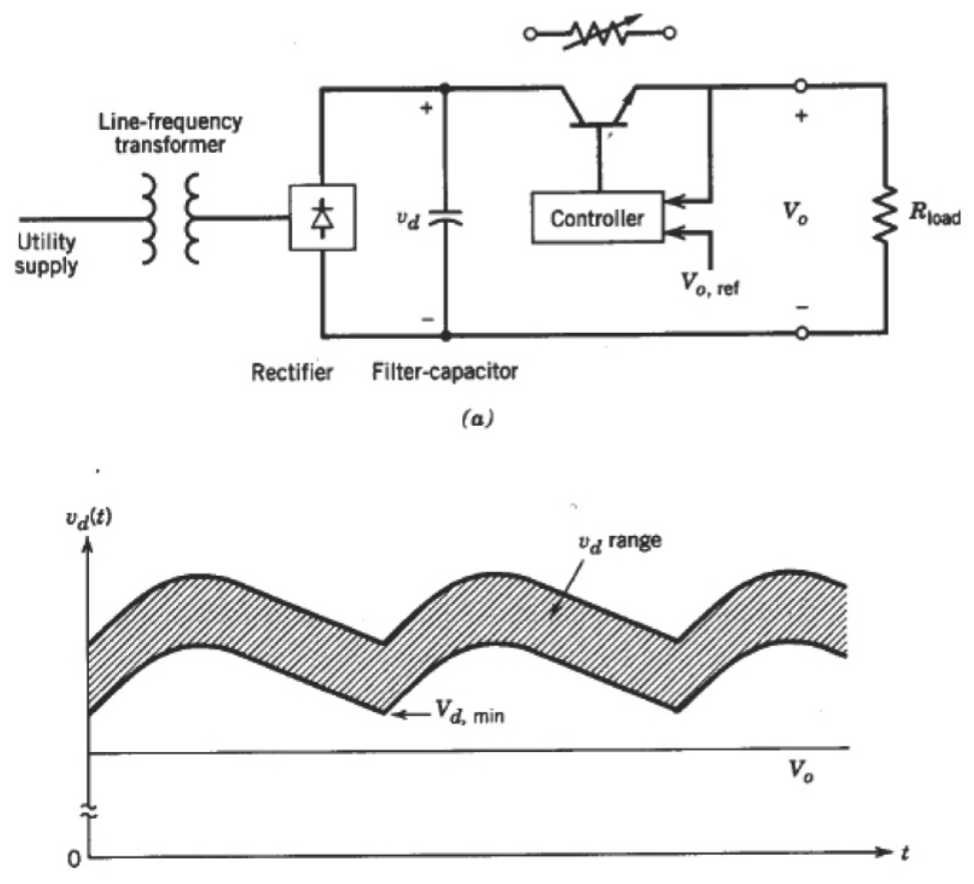
\includegraphics[scale=0.3]{ch5/1}
		\captionof{figure}{}
		\end{wrapfigure}
		Here we find the distribution of a linear supply. Its first level comprises a transformer that will also ensure galvanic isolation between the AC mesh and the DC mesh. Then there is a diode rectifier followed by a capacitor that will smooth the voltage. After the capacitor, the voltage is barely distorted (harmonics multiple of 100 Hz for a single-phase rectification) and its average value varies depending on the voltage of the supply and on the load. Thanks to the transformer we get a voltage $V_d$ slightly higher than the instruction $V_o$. The transistor will operate in its linear region and it will be controlled as a variable resistance. \\
		
		SMPS are more efficient, smaller and cheaper. The chopper operates at a frequency way higher than that of the grid (some kHz) $\Rightarrow$ the size of the magnetic components and the capacitors is greatly reduced. On the other hand, they are harder to control and the cutting induces distortions on voltages and currents. 
		
\section{Basic topologies: buck, boost and buck-boost}
	The three one-quadrant choppers are:
	\begin{itemize}
		\item[•] \textbf{buck converter} (hacheur dévolteur, series, step-down chopper, ...) 
		\item[•] \textbf{boost converter} (hacheur survolteur, parallel, step-up chopper, ...)
		\item[•] \textbf{buck-boost converter} (hacheur dévolteur-survolteur, ...)
	\end{itemize}
	\ \\
	We will focus on R loads with an smoothing capacity at the output. In addition, each converter has a switch (T), a free-wheeling diode (D), a self (L) and a capacitor (C). We will see a constant piecewise voltage $v_L(t)$ at the self's terminals and a sawtooth shaped current $i_L(t)$. For the buck and the boost converters we get the almost the same outputs if we put a brushed DC machine (RLE) at the output (where the machine operates as a motor) or at the input (where the machine operates as a dynamo). In these machines, the armature inductance will be enough to smooth the current (no need of extra inductors). 
	
	\subsection{Buck converter}	
	
		\begin{wrapfigure}[6]{l}{5.5cm}
		\vspace{-5mm}
		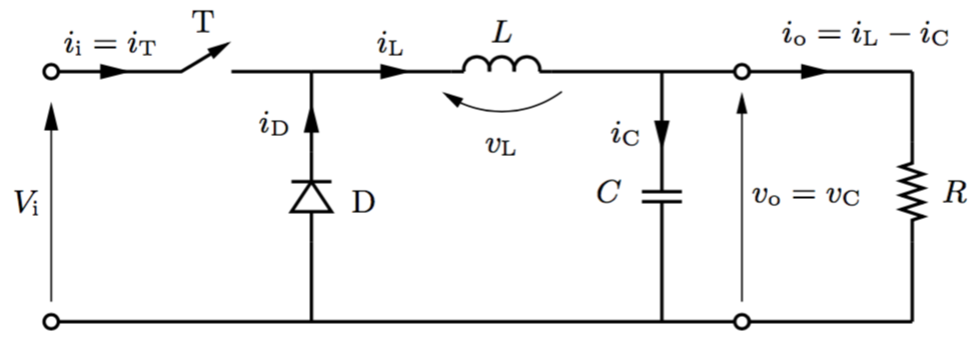
\includegraphics[scale=0.3]{ch5/2}
		\captionof{figure}{}
		\end{wrapfigure}
		In the figure, there is a buck converter with an LC filter and an R load with $V_o < V_i$, where $v_i= V_i$ is considered completely smooth. The current $i_1$ goes through the switch T and it is not smooth.  
		
		\ \\\\
		 		
		\begin{wrapfigure}[6]{r}{4.5cm}
		\vspace{-5mm}
		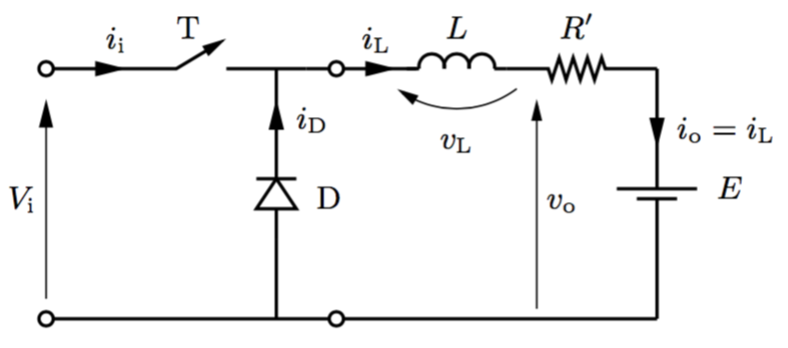
\includegraphics[scale=0.3]{ch5/3}
		\captionof{figure}{}
		\end{wrapfigure}	
		In this figure we find a system system equivalent to the previous one but with an RLE load. Under some hypothesis, the wave shapes, notably $v_L$ and $i_L$ are identical to the previous ones. From here onwards we will consider that the system has a PWM control. This way we will prove that the filter will work better (smoother output) when the commutation frequency $f_s$ of the PWM is big with respect to the cutoff frequency $f_c = 1/(2\pi\sqrt{LC})$. We can therefore 
		
		\begin{wrapfigure}[9]{l}{5.5cm}
		\vspace{0mm}
		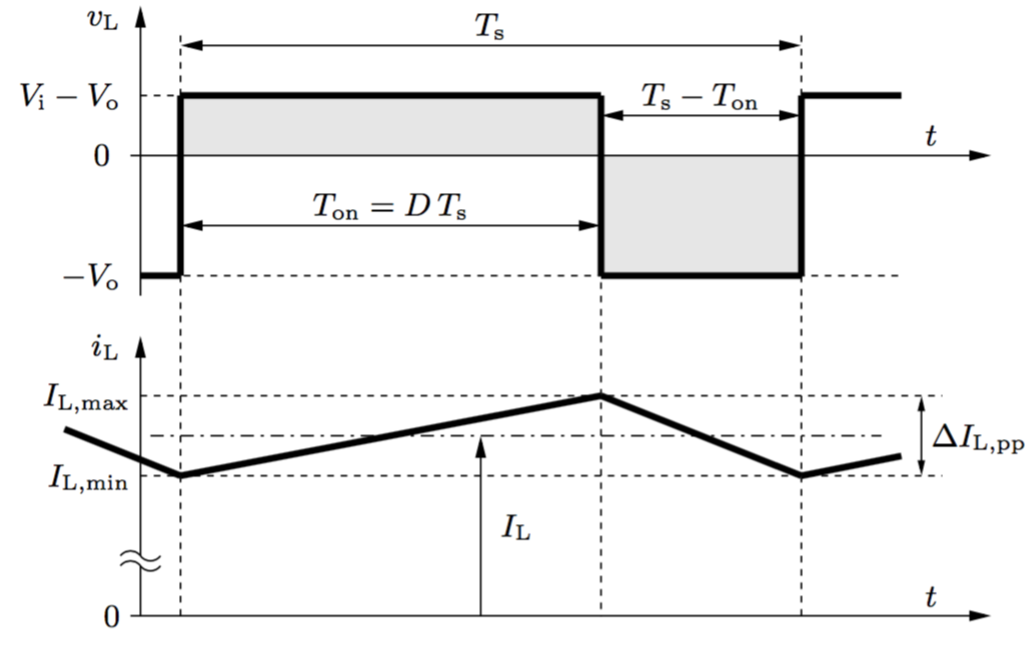
\includegraphics[scale=0.3]{ch5/4}
		\captionof{figure}{}
		\end{wrapfigure}	
		neglect the distortion of $v_o = v_C$, as well as the flaws of the components. We will use, once again, the duty cycle D (closing).When the switch (T) gets closed, D is in inverse-bias and $v_L = V_i - V_o>0$ corresponds to a current $i_L$ that grows with a slope $di_L/dt = (V_i -V_o)/L$.  \\
		
		If the switch is open, then $i_L$ is continuous and goes through D and $v_L = -V_o<0$ with a current $i_L$ that diminishes with a gradient $-V_o/L$. At steady-state $I_C = 0$, the average current output is therefore: 
		\begin{equation}
			I_o = I_L.
		\end{equation}
		If we make the hypothesis of continuous conduction, then $i_L$ has a sawtooth shape. At steady-state, the average voltage in the inductance $V_L = 0$, so:
		\begin{equation}
			DT_s(V_o-V_i) - (1-D)T_sV_o = 0 \qquad \Leftrightarrow \qquad V_o = DV_i
			\label{eq:5.2}
		\end{equation}
		This shows that $V_o$ ranges between 0 and $V_i$. Let's note that we find the same relation as that of the 2-quadrant half-bridge chopper, except here that relation is valid only if there is continuous conduction. If we consider that our components are ideal and the voltages are completely smooth, then we can get the relation $I_o/I_i$ by doing the power ratio:
		\begin{equation}
			V_iI_i = V_oI_o \qquad \Rightarrow \qquad \frac{I_o}{I_i}=\frac{1}{D}.
		\end{equation}		 
		As $v_L=  -V_o$ during $(1-D)T_s$, we have:
		\begin{equation}
			\Delta I_{L,pp} = I_{L,max}-I_{L,min} = (1-D)\frac{1}{f_sL}V_o = (1-D)D\frac{1}{f_sL}V_i
			\label{eq:5.4}
		\end{equation}
		
		\subsubsection{Ripple of the output voltage}
			\begin{wrapfigure}[8]{l}{6cm}
			\vspace{-5mm}
			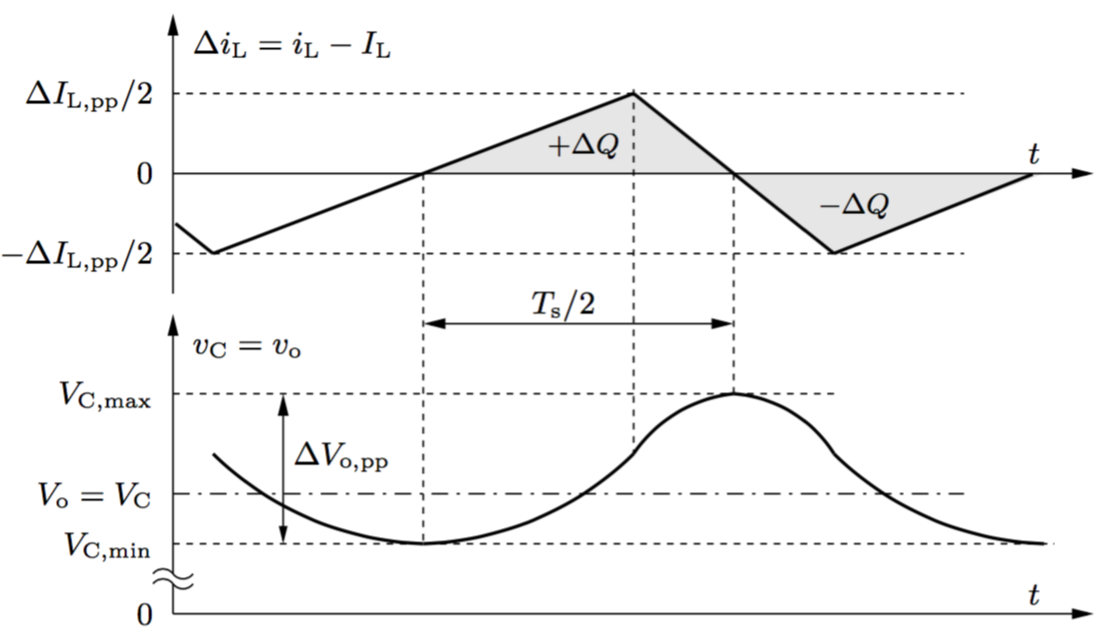
\includegraphics[scale=0.3]{ch5/5}
			\captionof{figure}{}
			\end{wrapfigure}	
			The current flowing through the capacitor is: 
			\begin{equation}
				i_C = i_L - \underbrace{i_o}_{\approx I_o = I_L}
			\end{equation}
			where we neglect the ripple of the current $i_o$ because it is way smaller than that of $i_L$. $i_C$ is thus equal to the distortion of $i_L$:
			\begin{equation}
				i_C = \Delta i_L = i_L -I_L.
			\end{equation}
			The charge of the capacitor will change as in the relation $q = \int i_C(t) \, dt$, and therefore $v_o = v_c = q/C$. They will vary around the average charge $Q$ and the average voltage $V_o = V_c = Q/C$ respectively.During a positive alternation of the current $i_C$, $v_o$ increases from $V_{C,min}$ until it reaches $V_{C,max}$ at the end of the alternation; the inverse process takes place during negative alternations. The taken or furnished charge $\Delta Q$ is the area: 
			\begin{equation}
				\Delta Q = \frac{1}{2}\frac{T_s}{2}\frac{\Delta I_{L,pp}}{2} = \frac{1}{8f_s}\Delta I_{L,pp} \qquad \Rightarrow \qquad \Delta V_{o,pp} = \frac{\Delta Q}{C} = \frac{1}{8f_sC}\Delta I_{L,pp}.
			\end{equation}
			With \eqref{eq:5.4} and $f_c = 1/2\pi \sqrt{LC}$, the relative ripple is: 
			\begin{equation}
				\frac{\Delta V_{o,pp}}{V_o} = \frac{1}{8}\frac{1}{f_s^2LC}(1-D) = \frac{\pi ^2}{2}\left(\frac{f_c}{f_s} \right)(1-D). 
			\end{equation}
			For a given D, we can reduce the ripple by increasing the switching frequency $f_s$ or the total LC. However, both means have their cons: more commutation losses and bigger, more expensive and heavier converters. 
			
		\subsubsection{Limit between continuous and discontinuous conduction}
			\begin{wrapfigure}[5]{r}{6.5cm}
			\vspace{-5mm}
			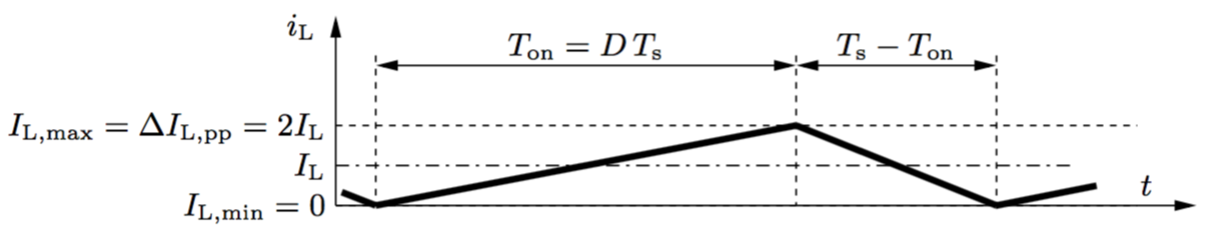
\includegraphics[scale=0.3]{ch5/6}
			\captionof{figure}{}
			\end{wrapfigure}
			We observe that R doesn't appear in the equations when current is continuous, but the capacity C does appear. For given $V_i, D$ and $f_s L$, the increase of the resistance generates a diminution of the current $I_L = I_o = V_o/R$ and its minimum $I_{L,min}=I_L - \Delta I_{L,pp}/2$. For a given R, we reach the limit between continuous and discontinuous conduction: $I_{L,min}=0$. At this limit we have:
			\begin{equation}
				I_{o,lim} = I_{L,lim} = \Delta I_{L,pp}/2 = (1-D)\frac{1}{2f_sL}V_o = (1-D)D\frac{1}{2f_sL}V_i.
			\end{equation}
			Let's introduce a reference for the average current:
			\begin{equation}
				I_{o,ref} = \frac{1}{8f_sL}V_i \qquad \Rightarrow \qquad I_{o,lim} = 4(1-D)DI_{o,ref}.
			\end{equation}
			
		\subsubsection{Discontinuous conduction}
			\begin{wrapfigure}[7]{l}{6cm}
			\vspace{0mm}
			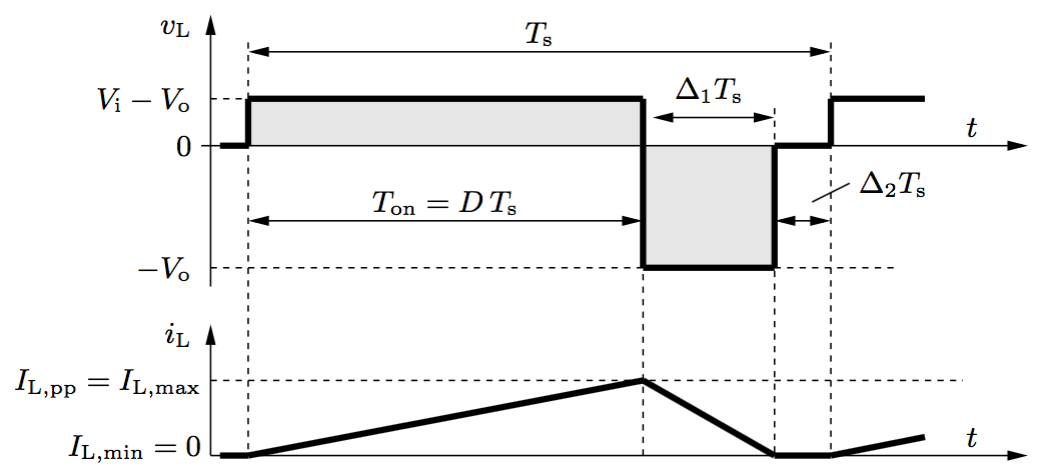
\includegraphics[scale=0.3]{ch5/7}
			\captionof{figure}{}
			\end{wrapfigure}	
			When conduction is discontinuous $i_L(t) = 0$ at the end of each commutation cycle (before closing again) and $v_L(t)$ will also become zero. \eqref{eq:5.2} is not valid anymore and $V_o$ will also depend on $I_o$. The commutation cycle consists of 3 intervals:
			\begin{equation}
				D + \Delta _1 + \Delta _2 = 1 \qquad where \qquad 0<\Delta < 1-D.
			\end{equation}
			
			At steady state $V_L = 0$ thus:
			\begin{equation}
				DT_s (V_i - V_o) - \Delta _1 T_s V_o = 0 \qquad \Leftrightarrow \qquad \frac{V_o}{V_i} = \frac{D}{D+\Delta _1} > D. 
			\end{equation}
			
			We ascertain that $V_o$ is bigger when current is discontinuous for given $V_i$ and $D$. The average output current will be:
			\begin{equation}
				I_o = I_L = I_{L,max}\frac{D+\Delta _1}{2}\qquad where \qquad I_{L,max} = D\frac{1}{f_sL}(V_i-V_o).
			\end{equation}
			
			\begin{wrapfigure}[8]{r}{4.5cm}
			\vspace{-5mm}
			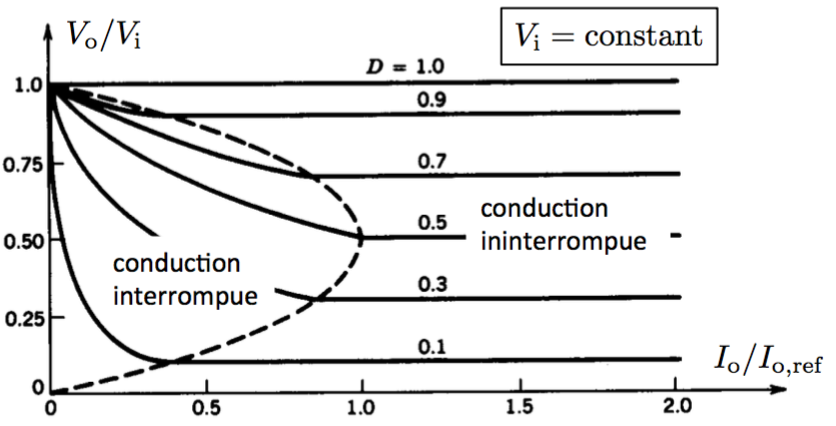
\includegraphics[scale=0.3]{ch5/8}
			\captionof{figure}{}
			\end{wrapfigure}
			If we combine the previous equations and $I_{o,ref}$ we get:
			\begin{equation}
				\frac{V_o}{V_i} = \frac{D^2}{D^2+\frac{1}{4}I_o/I_{o,ref}}.
			\end{equation}
			Here we show its dependence on $I_o/I_{o,ref}$ by considering a continuous and a discontinuous current zone. When current is discontinuous, $\frac{V_o}{V_i} = D$, $I_o$ won't affect that ratio. Remember that its characteristic with a resistive load R would be a line going through the origin in the figure:
			\begin{equation}
				\frac{V_o/V_i}{I_o/I_{o,ref}} = \frac{V_o}{I_o}\frac{I_{o,ref}}{V_i} = \frac{R}{8 f_s L}.
			\end{equation}
			
			For $R=\infty$ (no load), $V_o = V_i$ at steady-state. As a matter of fact, the capacitor cannot furnish a current to deplete its charge because there is no path for it go through. In fact, the capacitor could get charged during the transient state when there was still a load by a current $i_L\geq  0$, but without the load it cannot get rid of the charge. 
			
	\subsection{Boost converter}
		\begin{center}
		\begin{minipage}{0.45\textwidth}
			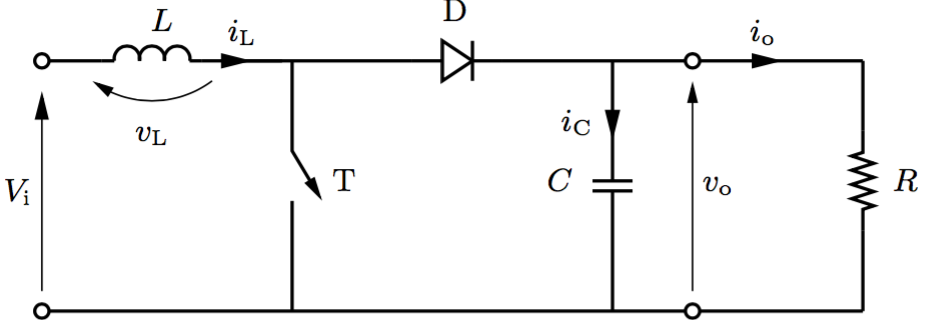
\includegraphics[scale=0.42]{ch5/9}
			\captionof{figure}{}
		\end{minipage}
		\begin{minipage}{0.45\textwidth}
			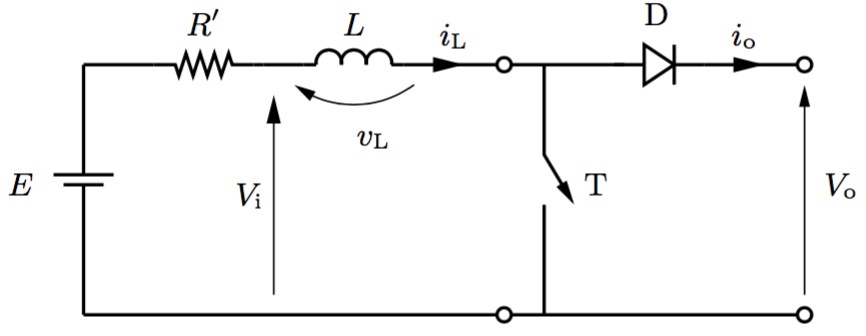
\includegraphics[scale=0.41]{ch5/10}
			\captionof{figure}{}
		\end{minipage}
		\end{center}
		
		\begin{wrapfigure}[7]{l}{5.5cm}
		\vspace{-5mm}
		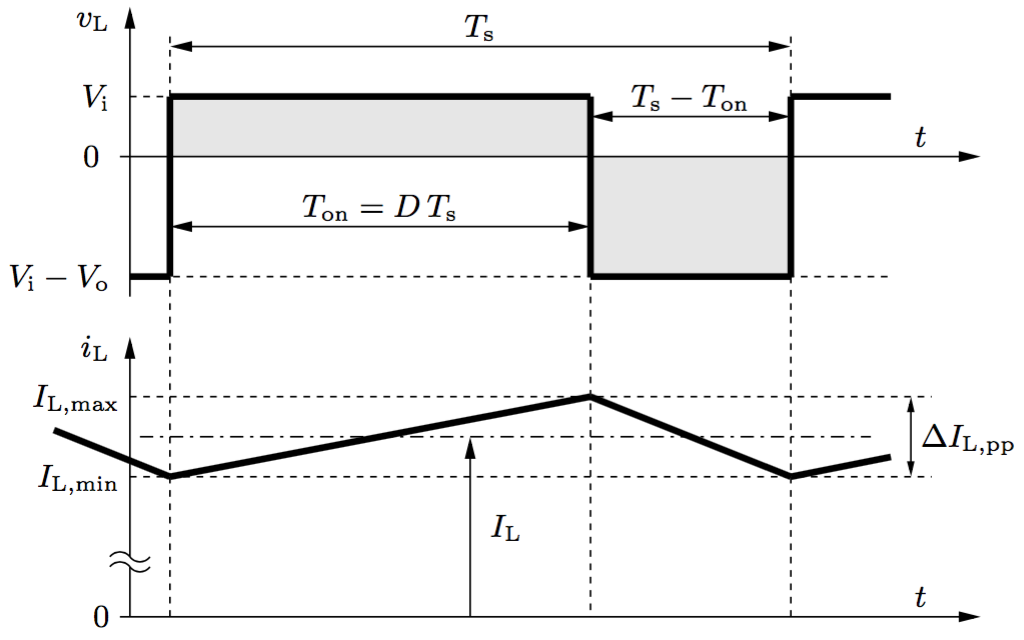
\includegraphics[scale=0.3]{ch5/11}
		\captionof{figure}{}
		\end{wrapfigure}	
		The device shown in the figure (left) is very similar to the buck converter. The only difference is the disposition of the components (the boost has a voltage smoothing capacitor). The figure on the right represents the case of a boost converter with a voltage source in the output and a RLE load in the input (brushed DC machine operating as a dynamo). 
		
		\ \\ The same way as before, the PWM control gives a sawtooth shaped current $i_L(t)$ when conduction is continuous. When the switch is closed, $v_D = -V_o$ and $v_L(t) = V_i >0$ and the current $i_L(t)$ grows with a slope $V_i/L$. When the witch is open, $v_L(t) = V_i - V_o < 0$ and the current $i_L$ flowing through the free-wheeling diode decreases with a slope $(V_i - V_o) /L$. As the average voltage over the inductor is zero:
		\begin{equation}
			DT_s V_i + (1-D)T_s (V-i-V_o) = 0 \qquad \Leftrightarrow \qquad V_o = \frac{1}{1-D}V_i. 
		\end{equation}
		We see that $V_o \geq V_i$ which justifies the name given to this chopper. 
		
		\begin{wrapfigure}[5]{l}{3.5cm}
		\vspace{-5mm}
		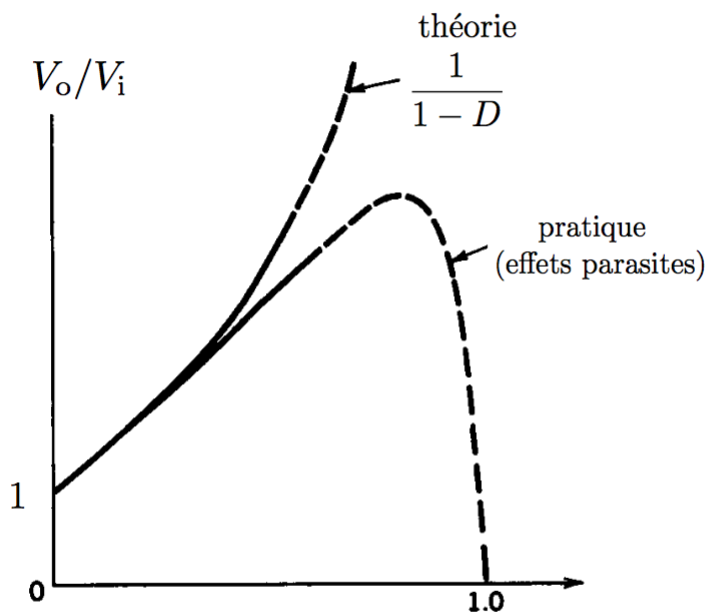
\includegraphics[scale=0.25]{ch5/12}
		\captionof{figure}{}
		\end{wrapfigure}
		This figure shows the theoretical characteristic and we see that its theoretical value $\rightarrow \infty$ if D $\rightarrow 1$. However, that doesn't happen in practice because of the parasitic effects of the non-ideal components (residual voltages of switches and diodes, inner resistances of the self and the capacitor, ...).   \\\\
		
	\subsection{Buck-boost converter}
		\begin{wrapfigure}[3]{r}{5.1cm}
		\vspace{-16mm}
		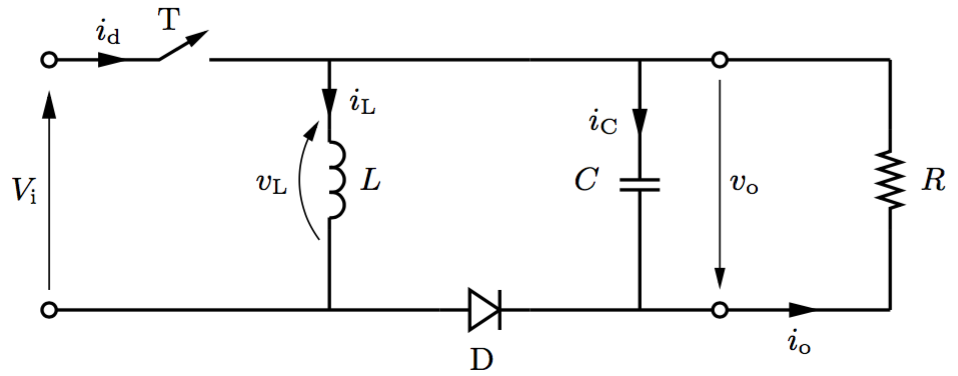
\includegraphics[scale=0.3]{ch5/13}
		\captionof{figure}{}
		\end{wrapfigure}
		Yet another distribution of the components gives the system in the figure, the buck-boost converter. In the figure there is also a bleeding capacitor and an R load. 
		
		\ \\
		\begin{wrapfigure}[8]{l}{4.5cm}
		\vspace{-5mm}
		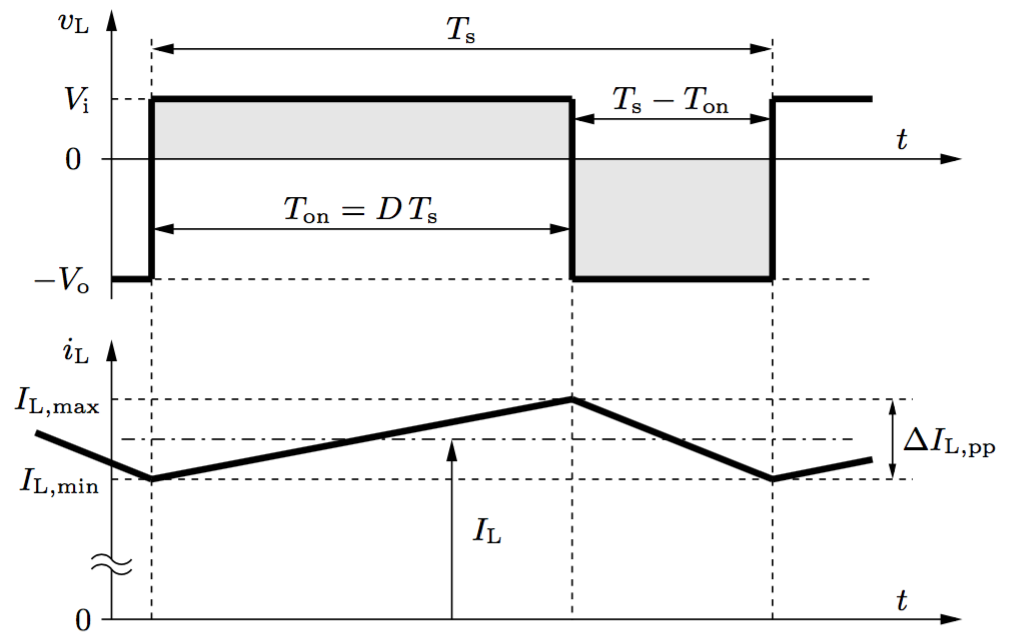
\includegraphics[scale=0.25]{ch5/14}
		\captionof{figure}{}
		\end{wrapfigure}	
		$i_L(t)$ has a sawtooth shape for continuous conduction. When the switch is closed, $v_L(t) = V_i$ and $i_L$ grows bigger. When T is open, $v_L = V_o$ because this time $V_o$ is inverted. Once again, for $V_L = 0$ when conduction is continuous: 
		\begin{equation}
			DT_s V_i - (1-D)T_s V_o = 0 \qquad \Leftrightarrow \qquad V_o = \frac{D}{1-D}V_i.
		\end{equation}
		We can have $V_o \leq V_i$ where $V_o \geq V_i$. For $D = 0.5$, $V_o =V_i.$ \\ 
		
		\begin{wrapfigure}[6]{r}{4.5cm}
		\vspace{-5mm}
		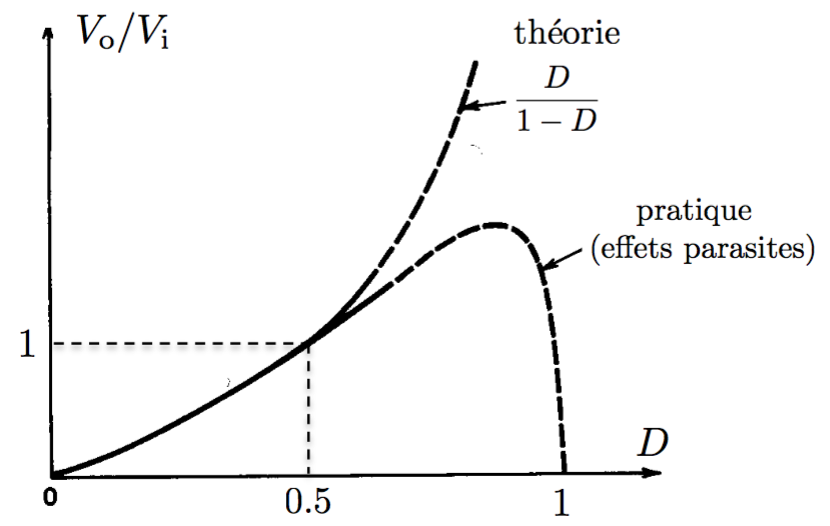
\includegraphics[scale=0.3]{ch5/15}
		\captionof{figure}{}
		\end{wrapfigure}
		Let's note that the inversion of $V_o$ might be an advantage. Right here we find the characteristic. In it we ascertain that the ratio $D/(1-D)$ is the result of setting a buck and a boost converter in series. However doing that is not a good idea because we would need twice as many components and thus we would double the weight, size, cost and losses of the device.

		
\section{Choppers with galvanic isolation - flyback converter}
	\begin{wrapfigure}[7]{l}{6cm}
	\vspace{-5mm}
	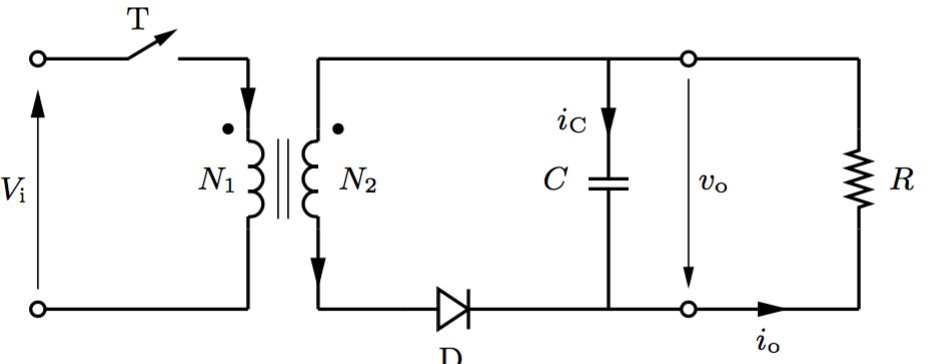
\includegraphics[scale=0.35]{ch5/16}
	\captionof{figure}{}
	\end{wrapfigure}
	Parasitic effects will be more relevant when the voltage difference becomes bigger. In addition, for a given power $V_oI_o = V_iI_i$. If we disregard losses, the biggest voltage amongst those two will determine the voltage capacity $V_{T,max}$ for a commutation period T. We find the maximum current capacity $I_{T,max}$ with the same method. We can conclude that the power capacity will be worst if the difference between $V_o$ and $V_i$ (and thus between $I_o$ and $I_i$) is big. In these cases, it's appropriate to add a high frequency \textbf{transformer} able to work properly at the commutation frequency $f_s$. The figure shows this kind of converter, the \textbf{flyback converter} (it's a buck-boost converter where the inductor is substituted by a transformer). If conduction is continuous, the relation between voltages is:
	
	\begin{equation}
		V_o = \frac{D}{1-D}\frac{N_2}{N_1} V_i.
	\end{equation}
	
	It is not a classic transformer. Firstly, it operates at high frequencies, which makes it smaller. Because of that we can use a ferrite core instead of superposed magnetic sheets. Secondly, it also works as an energy limiter (as the self we used to have did). That energy storage is possible only if the core has an air-gap. That's because the magnetic density of the air $\frac{1}{2}B^2/\mu$ ($\mu _0$) is bigger that that of the iron ($\mu \gg$).
